\section{Our First Interacting Theory Part II}
Last class, we looked at our first interacting QFT - we looked at an interaction term in the action, $S_{\text{int}} = -\frac{\lambda}{(3!)^2}\int d^D x \phi^3$. We worked perturbatively in the interaction, and found that we could find correlation functions in the interacting theory in terms of (harder, but computable) correlation functions in the free theory. We found that, if we look at the connected correlation functions:
\begin{equation}
    \avg{\phi(x)\phi(0)}_{\lambda, c} = \avg{\phi(x)\phi(0)} + \frac{i^2}{2}\left.\avg{\phi(x)S_{\text{int}}^2\phi(0)}\right|_{\text{no bubbles, connected}} + O(\lambda^3)
\end{equation}
i.e. that with connected correlators, disconnected and bubble diagrams had no contributions. This is in fact general. Connected correlators, which generically are defined as:
\begin{equation}
    \fd{^n}{(iJ)^n}\log Z[J]
\end{equation}
only receive contributions from connected Feynman diagrams.

\subsection{Symmetry Factors}
The two remaining diagrams that contributed ended up being diagram (A):
\begin{equation}
    G(x - x_2)G(x_2 - x_1)^2 G(x_1)
\end{equation}
\begin{center}
    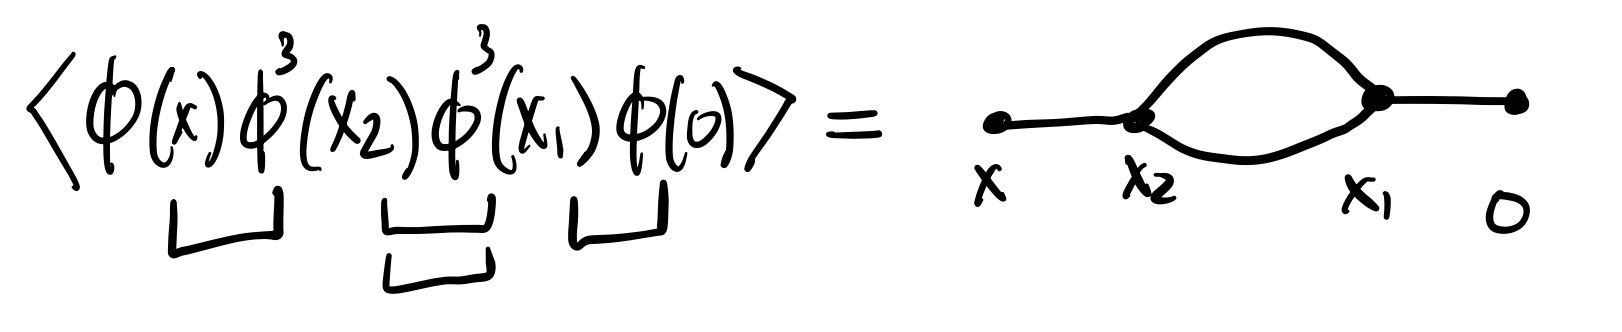
\includegraphics[scale=0.4]{Lectures/Figures/lec11-diag3.png}
\end{center}
and diagram (B):
\begin{equation}
    G(x - x_2)G(x_2 - x_1)G(0)G(x_2)
\end{equation}
\begin{center}
    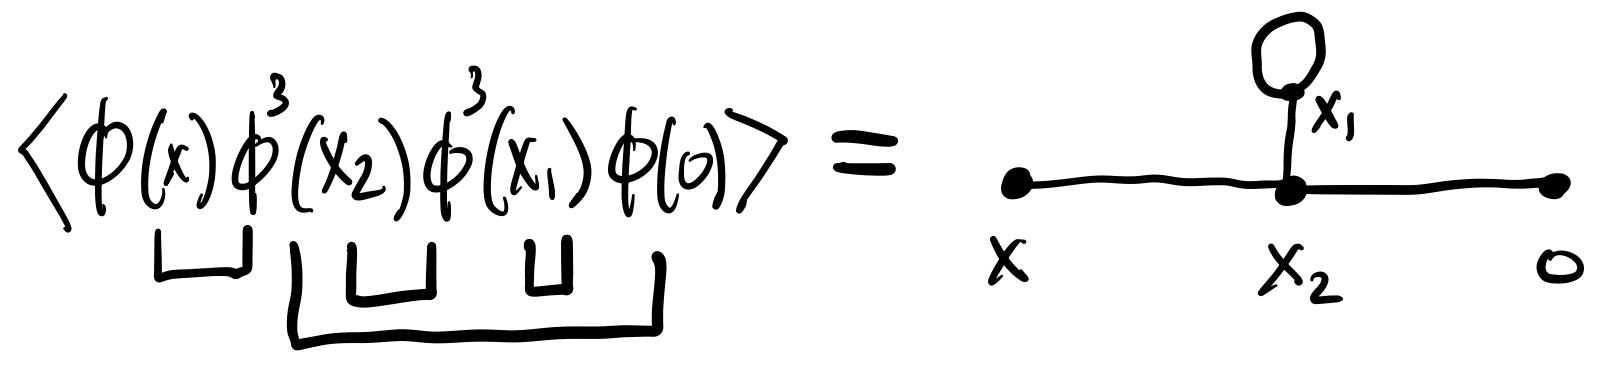
\includegraphics[scale=0.4]{Lectures/Figures/lec11-diag4.png}
\end{center}
which we will look at in more detail today. We'll study diagram (A), and we'll leave B for the problem set.

The contribution from all contractions is:
\begin{equation}
    \frac{i^2}{2}\frac{\lambda^2}{(3!)^2}\int_{x_1, x_2}\left.\avg{\phi(x)\phi^3(x_2)\phi^3(x_1)\phi(0)}_0\right|_{\text{no bubbles, connected}}
\end{equation}
We note that there are several Wick contractions that lead to the same diagram. All choices give the same diagram, but we need to take into account the symmetry factor of the diagram (how many choices of contractions). Let's think about the symmetry factor for (A). 
\begin{itemize}
    \item First, we want to contract $\phi(x)$ with fields at $x_1$ or at $x_2$. This gives us a factor of 2.
    \item Further, after choosing one of $x_1$ or $x_2$, we have a choice of three fields to contract with (as we have $\phi(x_1)^3/\phi(x_2)^3$). This gives a factor of 3.
    \item Now, for diagram A, $\phi(0)$ must be contracted with the remaining one of $x_1/x_2$. There are then 3 possible fields for it to be contracted with, giving a factor of 3.
    \item We have two remaining fields each in $\phi(x_1), \phi(x_2)$. We don't want to contract $\phi(x_1)$ with itself as that gives a disconnected diagram. So, there are two possible contractions between the two $\phi(x_1)$s and the two $\phi(x_2)$s. This gives a factor of 2.
\end{itemize}
In total, the symmetry factor of diagram (A) is:
\begin{equation}
    2 \cdot 3 \cdot 3 \cdot 2 = 36 = (3!)^2
\end{equation}
Which cancels out the $(3!)^2$ in the denominator, and so the A part of the correlator is:
\begin{equation}
    (A) =  -\frac{\lambda^2}{2}\int_{x_1, x_2}G(x - x_2)G(x_2 - x_1)^2 G(x_1)
\end{equation}

Physically, we can view this as the propogation in spacetime sketched below:

\begin{figure}[htbp]
    \centering
    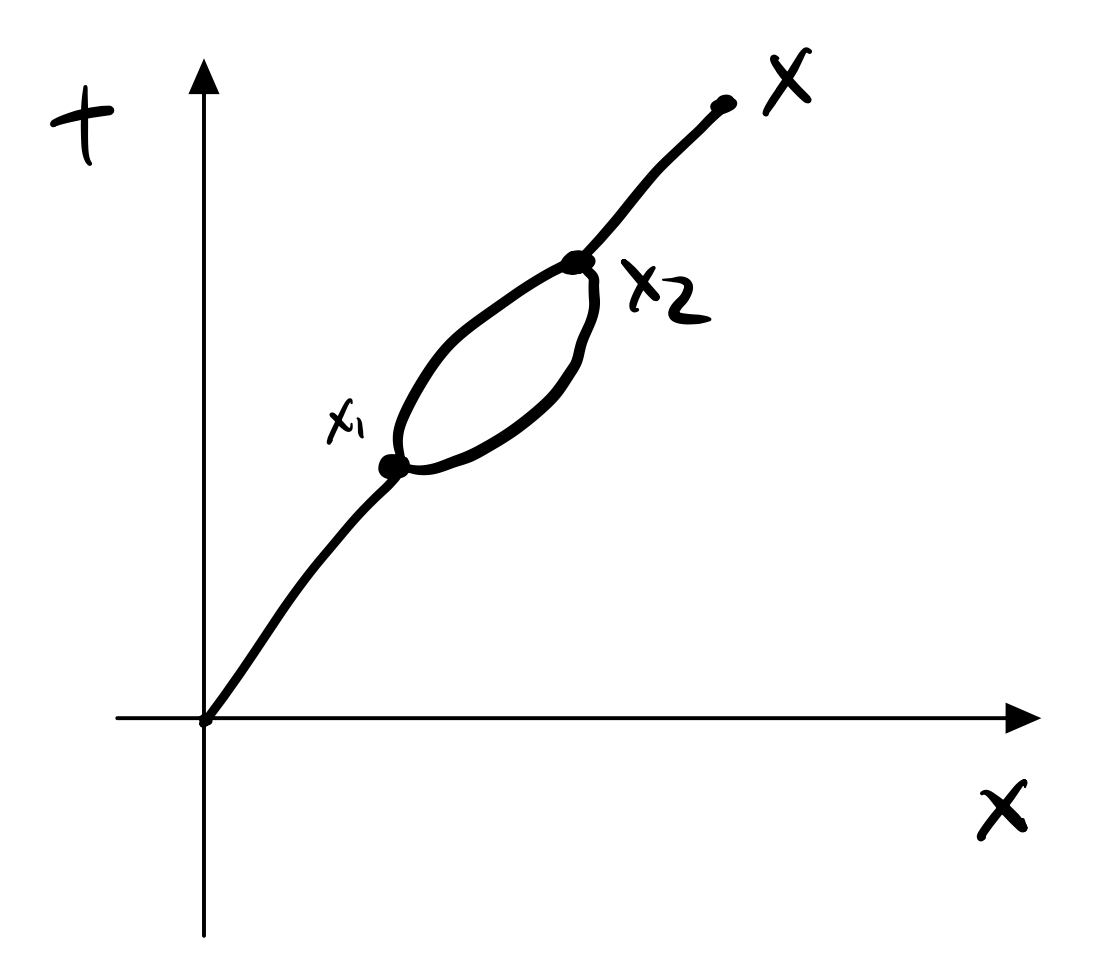
\includegraphics[scale=0.3]{Lectures/Figures/interactingprop-spacetime.png}
    \caption{Picture of the interacting diagram as a particle propagating in spacetime.}
    \label{fig:interactingprop-spacetime}
\end{figure}

It ``looks like'' the particle splits into two at $x_1$ due to the interaction, and then recombines at $x_2$. Compare this to the free theory, where the particle just propagates from $0$ to $x$.

\subsection{Going to Momentum Space}
We have nice expressions for these Green's functions in momentum space:
\begin{equation}
    G(x_1) = \int \frac{d^Dp_1}{(2\pi)^D}e^{ip_\mu x^\mu_1}G(p_1) = \int \frac{d^Dp_1}{(2\pi)^D}e^{ip_\mu x^\mu_1} \frac{-i}{p_1^2 + m^2 - i\e}
\end{equation}
So Fourier transforming each of the Green's functions in the (A) expression:
\begin{equation}
    (A) = -\frac{\lambda^2}{2}\int d^{D}x_1 d^D x_2\int \frac{d^Dp_1d^Dp_2d^Dp_3d^Dp_4 }{(2\pi)^{4D}} e^{ip_4(x - x_2)}e^{ip_3(x_2- x_1)}e^{ip_2(x_2 - x_1)}e^{ip_1(x_1)}G(p_4)G(p_3)G(p_2)G(p_1)
\end{equation}
The $x_1$ integral gives:
\begin{equation}
    (2\pi)^D \delta^D(p_1 - p_2 - p_3) \implies p_3 = p_1 - p_2
\end{equation}
and the $x_2$ integral gives:
\begin{equation}
    (2\pi)^d \delta^D(p_4 - p_2 - p_3) \implies p_4 = p_2 + p_3 = p_1
\end{equation}
We are thus left with:
\begin{equation}
    (A) = -\frac{\lambda^2}{2}\int_{p_1p_2}e^{ip_1 x}G(p_1)G(p_2)G(p_1 - p_2)G(p_1) = \delta G(x)
\end{equation}
Fianlly, Fourier transforming the result:
\begin{equation}
    \delta G(p) = \int d^Dx e^{-ipx}\delta G(x)
\end{equation}
which gives a factor of $(2\pi)^D \delta(p_1 - p)$, we obtain:
\begin{equation}
    \delta G(p) = -\frac{\lambda^2}{2}\int \frac{d^Dp_2}{(2\pi)^D}G(p)G(p_2)G(p - p_2)G(p) = -\frac{\lambda^2}{2}G(p)^2\int \frac{d^Dp'}{(2\pi)^D}G(p')G(p -p')
\end{equation}
This expression suggests a momentum space interpretation of the Feynman rules. A particle comes in with momentum $p$, then splits into to particles with momenta $p'$ and $p - p'$ (such that the momentum is conserved at the vertex), recombining into a particle with momentum $p$ at the end of the loop. The loop momentum $p'$ is integrated over. More consisely, we can say that the ``momentum space Feynman rules'' are:
\begin{itemize}
    \item Momentum are conserved at vertices of momentum space Feynman diagrams.
    \item Loop momentum are integrated over.
\end{itemize}
Instead of learning a bunch of Feynman rules/diagrams by heart (as might be the older approach to QFT), it's better to know how to derive them using the path integral, as there are many interesting known QFTs!

\begin{figure}[htbp]
    \centering
    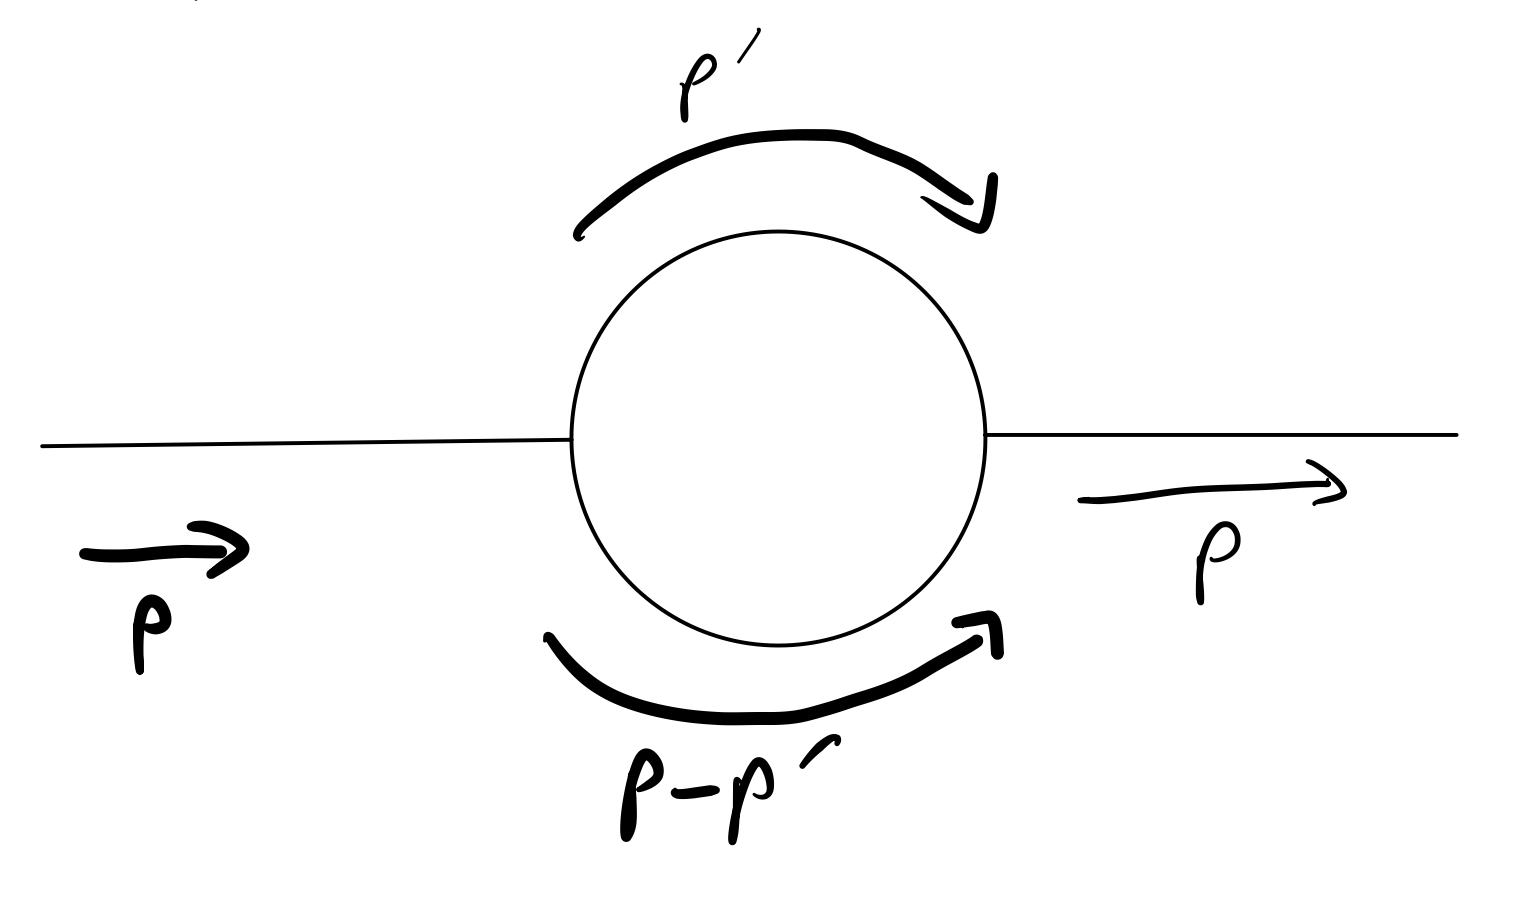
\includegraphics[scale=0.3]{Lectures/Figures/interactingprop-momentum.png}
    \caption{Picture of the interacting diagram as a particle propagating in momentum space.}
    \label{fig:interactingprop-momentum}
\end{figure}

\subsection{Self-Energy and Computing the Loop Integral}
Before trying to compute this integral, there is a useful parameterization of this correction in terms of a (small) ``self-energy\footnote{not a particularly great name}'' $\Pi$. In terms of this, we can write the interacting Green's function as:
\begin{equation}
    G_{\text{int}}(p) = G(p) + \delta G(p) = \frac{-i}{p^2 + m^2 + \Pi(p)} = \frac{-i}{p^2 + m^2}\frac{1}{1 - \frac{\Pi(p)}{p^2 + m^2}} \approx \frac{-i}{p^2 + m^2}\left(1 + \frac{\Pi(p)}{p^2 + m^2} + \ldots \right)
\end{equation}
at this point we aren't justified in keeping the higher order terms, because we've only worked to $O(\lambda^2)$ and the higher order terms are in higher powers of $\lambda$. But, to linear order in the self energy (which is $O(\lambda^2)$):
\begin{equation}
    G_{\text{int}}(p) = G(p) + G(p)^2 i\Pi(p)
\end{equation}
i.e. we have re-packaged the correction in terms of $\Pi(p)$. So:
\begin{equation}
    \Pi(p) = \frac{i\lambda^2}{2}\int \frac{d^Dp'}{(2\pi)^D}G(p')G(p - p')
\end{equation}
Which can be viewed as just the loop part of the momentum-space Feynman diagram. We know the free Feynman propagators, and so can write the above as:
\begin{equation}
    \Pi(p) = \frac{i\lambda^2}{2}\int \frac{d^Dp'}{(2\pi)^D}\frac{-i}{p'^2 + m^2 - i\e}\frac{-i}{(p - p')^2 + m^2 - i\e}
\end{equation}
The computation is technical, but it will be our first concrete/worked out result in interacting QFT, so it wil be worth it.

We consider the following recipe for evaluating loop integrals:
\begin{itemize}
    \item If the integrals involve more than one propagator (in our case, 2), we can use Feynman parameters to simplify down into one denominator.
    \item The $i\e$ appearing in the denominators can be slightly hard to work with. We will ``Wick rotate'', i.e. perform a contour deformation in the frequency $p_0'$. This integral has poles at (roughly) $p_0' = \pm \sqrt{\v{p}'^2 + m^2 - i\e}$. If we Taylor expand the $i\e$, the poles are at $p_0' = \pm \sqrt{\v{p}'^2 + m^2} \mp i\e$. If we look at this in the complex plane, we can consider the contour:
    
    \begin{figure}[htbp]
        \centering
        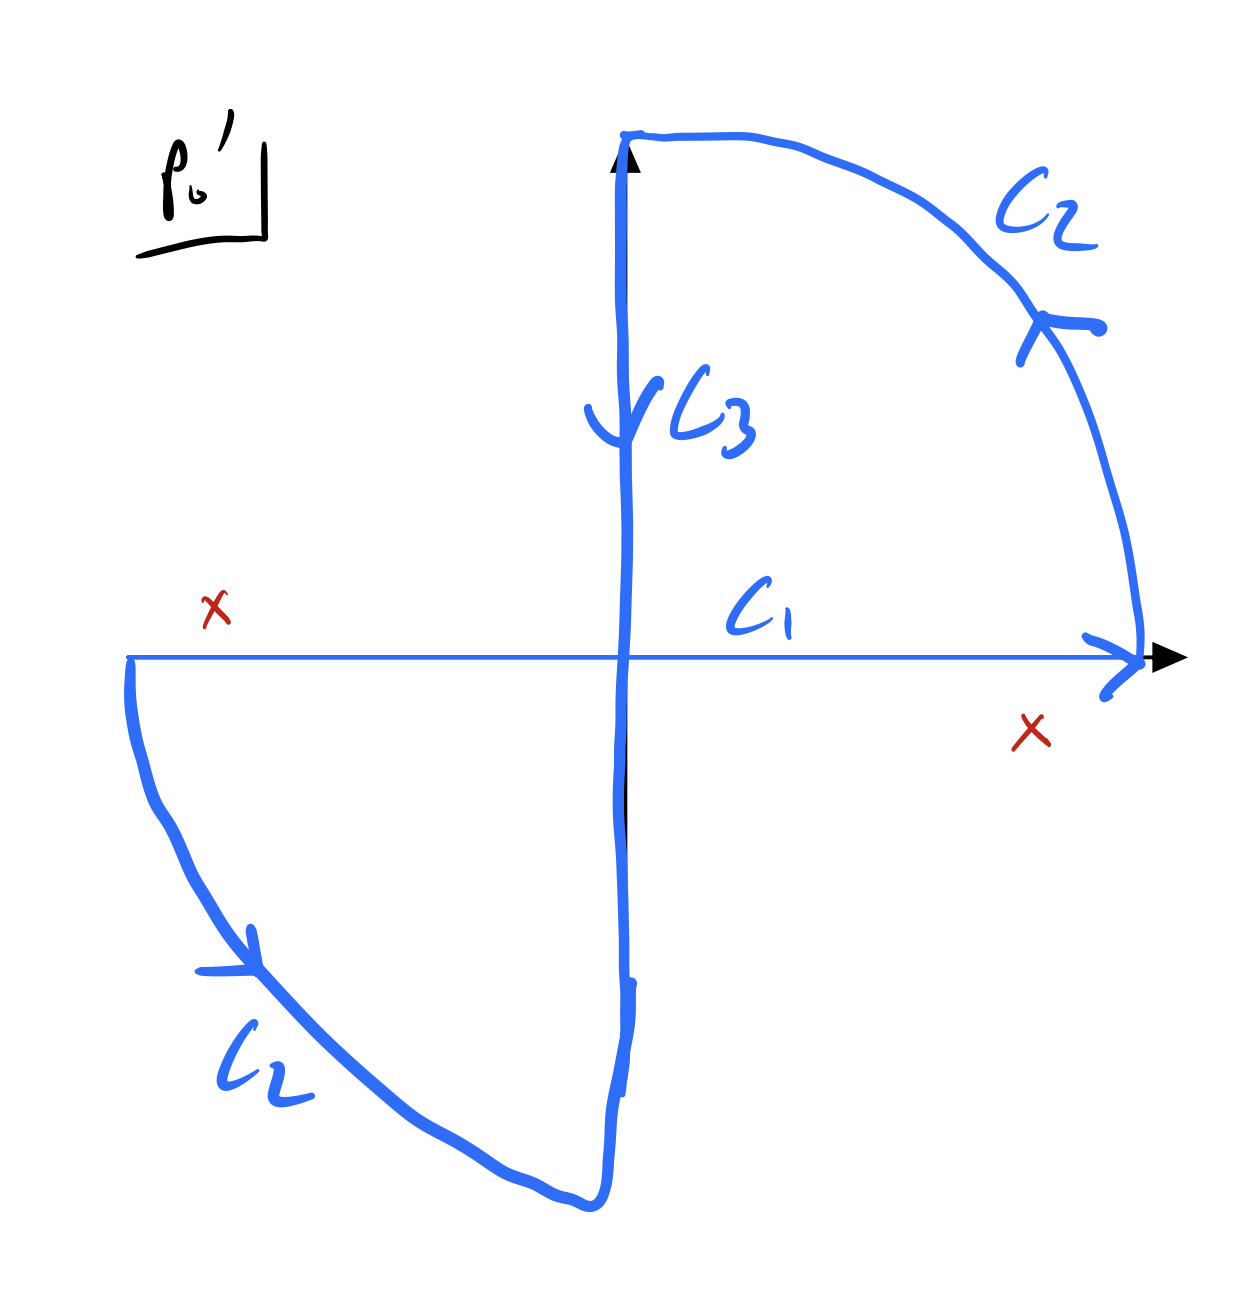
\includegraphics[scale=0.3]{Lectures/Figures/butterflycontour.png}
        \caption{Contour integral of $p_0'$ in $\CC^2$, which will allow us to write the desired integral (along the real axis) in terms of a ``Wick rotated'' integral along the imaginary axis.}
        \label{fig:butterflycontour}
    \end{figure}

    Then, we find that (since the contour contains no poles):
    \begin{equation}
        \int_{C_1 \cup C_2 \cup C_3} dp_0' (\ldots) = 0
    \end{equation}
    Thus, rephrasing this in terms of the integral that we want, i.e. that over $C_1$:
    \begin{equation}
        \Pi(p) = \int_{C_1}p_0' (\ldots)  = -\int_{C_2} dp_0'(\ldots) - \int_{C_3} dp_0'(\ldots).
    \end{equation}
    as we send the $C_2$ contour to infinity, it will vanish, and so:
    \begin{equation}
        \Pi(p) = -\int_{C_3} dp_0'(\ldots) = \int_{+i\infty}^{-i\infty}dp_0' (\ldots)
    \end{equation}
    Along this whole contour, $p_0'$ is imaginary, so let us do the change of variable $p_0' = ip_0'^E$:
    \begin{equation}
        \Pi(p) = i\int_{-\infty}^\infty dp_0'^E (\ldots)
    \end{equation}
    so far it seems like we've made the problem no better, no worse. Just integrating along a different axis. But - the resulting integral will turn out to be much nicer! This is because:
    \begin{equation}
        p'^2 = p_\mu' p'^\mu = -p_0'^2 + p_i'^2 = (p_0'^E)^2 + p_i'^2 = p_E^2
    \end{equation}
    which is just the Euclidean norm in $D$ dimensions! I.e. we are working in regular space, not Minkowski (where the $-$ sign on the time component can make our lives a bit more complicated).
\end{itemize}

Alright, we've laid out the steps, let's go through the integral! we want to compute:
\begin{equation}
    \Pi(p) = \frac{i\lambda^2}{2}\int \frac{d^Dp'}{(2\pi)^D}\frac{-i}{p'^2 + m^2 - i\e}\frac{-i}{(p - p')^2 + m^2 - i\e}
\end{equation}
We do a trick to put this over a single denominator. We use the fact that:
\begin{equation}
    \begin{split}
        \int_0^1 dx \frac{1}{[xA + (1-x)B]^2} = \int_0^1 dx \frac{1}{(x(A - B) + B)^2} &=\left.-\frac{1}{(A-B)}\frac{1}{x(A - B) + B}\right|_0^1 
        \\ &= \frac{1}{A-B}\left(\frac{1}{B} - \frac{1}{A}\right) = \frac{1}{A-B}\frac{A-B}{A+B} = \frac{1}{AB}
    \end{split}
\end{equation}
Thus, applying this identity to the above, with:
\begin{equation}
    \begin{split}
        A &= (p' - p)^2 + m^2 - i\e
        \\ B &= p'^2 + m^2 - i\e
    \end{split}
\end{equation}
We obtain:
\begin{equation}
    \Pi(p) = -\frac{i\lambda^2}{2}\int_0^1 dx\int_{p'}\frac{1}{(x[(p' - p)^2 + m^2 - i\e] + (1-x)[p'^2 + m^2 - i\e])^2}
\end{equation}
Simplifying the denominator:
\begin{equation}
    \begin{split}
        \Pi(p) &= -\frac{i\lambda^2}{2}\int_0^1 dx\int_{p'} \frac{1}{[m^2 - i\e + p'^2 - 2p\cdot p'x + p^2x]^2} 
        \\ &= -\frac{i\lambda^2}{2}\int_{p'} \frac{1}{[(p' - xp)^2 + m^2 + p^2x(1-x) - i\e]^2}
        \\ &= -\frac{i\lambda^2}{2}\int_0^1 dx \int_q \frac{1}{(q^2 + \Delta - i\e)^2}
    \end{split}
\end{equation}
where in the second equality we complete the square and in the third equality we introduce a new variable of integration $q = p' - xp$ and define $\Delta = m^2 + p^2x(1-x)$ which does not depend on $q$. Now, this integral has a simple pair of poles, and we should be able to use the Wick rotation trick. Let us do it; substitute $q_0 \to iq_0^E$, so:
\begin{equation}
    \Pi(p) = \frac{\lambda^2}{2}\int_0^1 dx \int \frac{d^Dq_E}{(2\pi)^D} \frac{1}{(q_E^2 + \Delta - i\e)^2}
\end{equation}
where $q_E^2 = (q_E^0)^2 + (q_E^i)^2$ is the regular Euclidean norm. Let us go into spherical coordinates to evaluate this, as we observe that there is nothing in the integral that depends on the angles, only the magnitude of $q_E$:
\begin{equation}
    \Pi(p) = \frac{\lambda^2}{2} \int_0^1 dx \int \frac{dq_E q_E^{D-1}d^{D-1}\Omega}{(2\pi)^D}\frac{1}{(q_E^2 + \Delta - i\e)^2} = \frac{\lambda^2}{2} \frac{S_{D-1}}{(2\pi)^D}\int_0^1 dx \int_0^\infty q_E^{D-1}\frac{1}{(q_E^2 + \Delta - i\e)^2}
\end{equation}
where $S_{D-1}$ is the surface area of the unit $n$-sphere, i.e. $S_1 = 2\pi$, $S_2 = 4\pi$, $S_3 = 2\pi^2$. We can further simplify because the $\e$ is no longer relevant, it just was there to tell us how to Wick-rotate. Thus:
\begin{equation}
    \Pi(p) = \frac{\lambda^2}{2}\frac{S_{D-1}}{(2\pi)^D}\int_0^1 dx \int_0^\infty \frac{dq_E q_E^{D_1}}{(q_E^2 + \Delta)^2}
\end{equation}
So just 2 more integrals to go!

BUT now tragedy strikes. This integral actually diverges for $D \geq 4$ (for $D = 4$, we can see that it goes as $\log(q_E)$, and powers of $q_E$ for $D >4$). This is what is known as an ultraviolet divergence\footnote{Be thankful that you live in the 21st century, where we understand these completely!} To resolve this, let us introduce a sharp ultraviolet cutoff $\Lambda$:
\begin{equation}
    \int_0^{\infty} dq_E \to \int_0^\Lambda dq_E
\end{equation}
Then we obtain (in $D = 4$):
\begin{equation}
    \Pi(p) = \frac{\lambda^2}{2}\frac{2\pi^2}{(2\pi)^4}\int_0^1 dx \int_0^\Lambda dq_E \frac{q_E^2}{(q_E^2 + \Delta)^2}q_E
\end{equation}
Then we find:
\begin{equation}
    \int_0^\Lambda dq_E \frac{q_E^2}{(q_E^2 + \Delta)^2}q_E = \left. \frac{1}{2}\left(\frac{\Lambda}{q_E^2 + \Delta} + \log(q_E^2 + \Delta)\right)\right|_{0}^\Lambda = \frac{1}{2}\left(\log(\Lambda^2 + \Delta) + \frac{\Delta}{\Lambda^2 + \Delta} - \frac{1}{2}(1 + \log \Delta)\right)
\end{equation}
So, keeping in mind that $\Lambda$ is very large and keeping only the dominant terms in $\Lambda$, i.e.:
\begin{equation}
    \log(\Lambda^2 + \Delta) + \frac{\Delta}{\Lambda^2 + \Delta} \approx \log\Lambda^2 + O(\frac{\Delta}{\Lambda^2})
\end{equation}
we find:
\begin{equation}
    \Pi(p) = \frac{\lambda^2}{(4\pi)^2}\int_0^1 dx \left(\frac{1}{2}\log\Lambda^2 - \frac{1}{2} - \frac{1}{2}\log\Delta\right).
\end{equation}
Let's focus on the UV divergent $\log \Lambda$ piece:
\begin{equation}
    \left.\Pi(p)\right|_{\text{div}} = \frac{\lambda^2}{(4\pi)^2}\int_0^1 dx \log\Lambda = \frac{\lambda^2}{(4\pi)^2}\log \Lambda
\end{equation}
recall that:
\begin{equation}
    G_{\text{int}}(p) = \frac{-i}{p^2 + m^2 - \Pi(p)} = \frac{-i}{p^2 + m^2 - \lambda^2\frac{\log \Lambda}{(4\pi)^2}}
\end{equation}
this corresponds to a (momentum-independent) shift in the mass term. In the interacting theory, the physical pole is no longer simply given by the bare mass. The physical mass that the experimentalist measures now appears to be regulator-dependent:
\begin{equation}
    m_{\text{phys}}^2 = m^2 -\lambda^2\frac{\log \Lambda}{(4\pi)^2}
\end{equation}
This might sound upsetting, and Luca is going to leave this to sit with us for the weekend. But, next week we will resolve it, beautifully!